\chapter{Proprietà magnetiche della materia}

In questo capitolo andremo a trattare come i campi magnetici agiscono sui mezzi \\

Iniziamo dando una descrizione fenomenologica: consideriamo un solenoide rettilineo disposto con l'asse verticale e sospendiamo tramite una molla campioni di vari materiali aventi aventi piccole dimensioni. 

\begin{figure} [h]
    \centering
    \begin{subfigure}{0.45\textwidth}
        \centering
        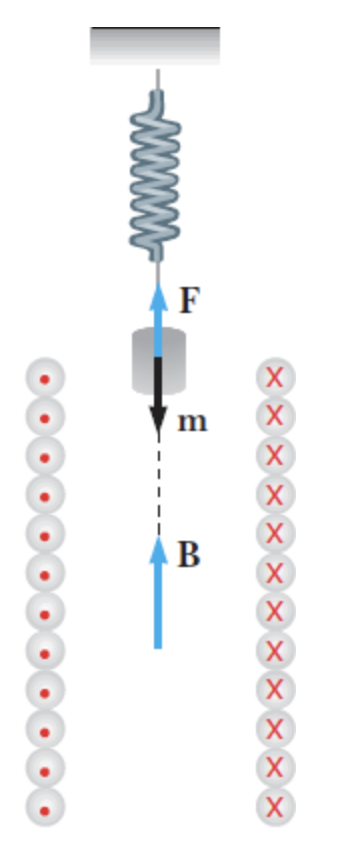
\includegraphics[width=0.5\linewidth]{figure/image52.png}
        \caption{Forza repulsiva}
        \label{fig:placeholder}
    \end{subfigure}
    \hfill
    \begin{subfigure}{0.45\textwidth}
        \centering
        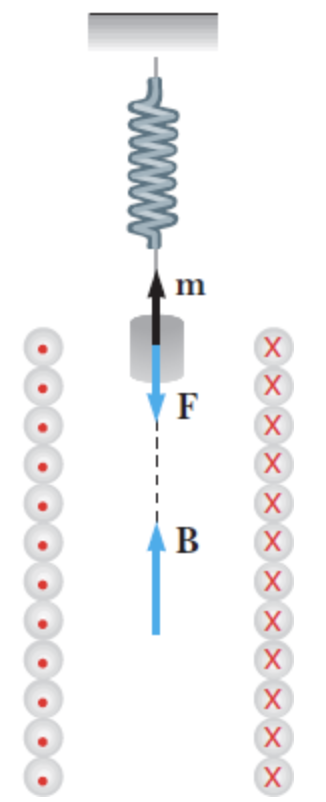
\includegraphics[width=0.5 \linewidth]{figure/image53.png}
        \caption{Forza attrattiva}
    \end{subfigure}
    \caption{Materiali sospesi soggetti al campo magnetico del solenoide}
\end{figure}

Quando nel solenoide circola corrente si osserva che su ciascun campione viene esercitata una forza. Alcuni campioni sono attratti verso l'interno, altri respinti verso l'esterno e ciò indipendentemente dal verso del campo magnetico. \\

Questo risultati si interpretano supponendo che alcune sostanze, sottoposte all'azione di un campo magnetico, acquistino un momento magnetico $\mathbf{m}$ parallelo e concorde a $\mathbf{B}$, mentre in altre $\mathbf{m}$ è parallelo e discorde a $\mathbf{B}$. \\

In base alle caratteristiche sperimentali descritte si può procedere a una suddivisione in tre classi alle quali, come vedremo in seguito, corrispondono diversi meccanismi microscopici di formazione del momento magnetico in presenza di un campo magnetico.

\begin{itemize}
    \item \emph{Sostanze diamagnetiche} \mkeyword{Sostanze diamagnetiche}
\end{itemize}

Sono dette diamagnetiche le sostanze che vengono respinte dal solenoide: la magnetizzazione è opposta al campo magnetico $\mathbf{B}$ esterno ed è ad esso proporzionale; l'effetto non dipende dalla temperatura, salvo poche eccezioni. È questa la classe più ampia a cui appartiene la maggior parte delle sostanze.

\begin{itemize}
    \item \emph{Sostanze paramagnetiche} \mkeyword{Sostanze paramagnetiche}
\end{itemize}

Si chiamano paramagnetiche le sostanze che vengono attratte dal solenoide, quelle cioè in cui la magnetizzazione è concorde al campo magnetico. Si trova che in generale l'effetto aumenta al diminuire della temperatura, ma ci sono svariate eccezioni. In tutti i casi si tratta di forze piuttosto piccole, alle temperature ordinarie.

\begin{itemize}
    \item \emph{Sostanze ferromagnetiche} \mkeyword{Sostanze ferromagnetiche}
\end{itemize}

Infine sono dette ferromagnetiche le sostanze che sono attratte fortemente verso la zona in cui il campo magnetico è maggiore; anche in questi campioni la magnetizzazione è concorde al campo magnetico, però la relazione tra $\mathbf{m}$ e $\mathbf{B}$ non è lineare e nemmeno univoca. Inoltre di norma i campioni rimangono magnetizzati anche dopo che il campo è stato rimosso, cosa che non accade con le sostanze diamagnetiche e paramagnetiche.

\section{Magnetizzazione}

In presenza di un campo magnetico, la materia si magnetizza, cioè gli atomi o le molecole del materiale acquistano sotto l'azione del campo $\mathbf{B}$ un momento magnetico medio $<\mathbf{m}>$ orientato parallelamente a $\mathbf{B}$. 

\begin{figure} [h]
    \centering
    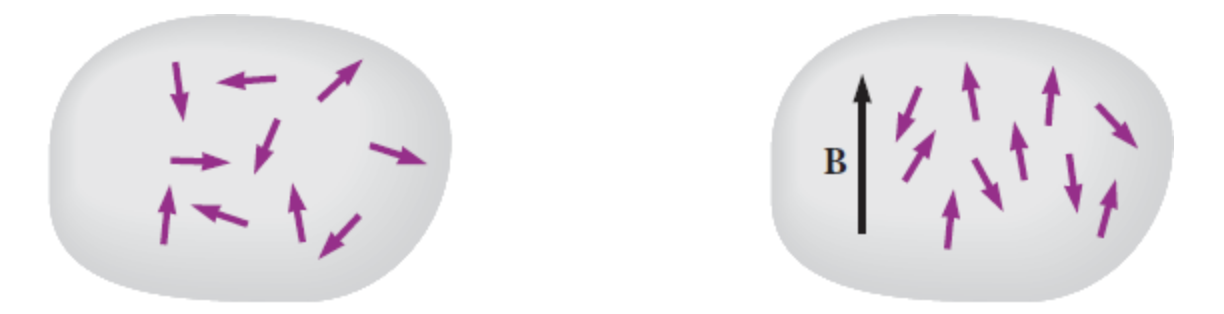
\includegraphics[width=0.8\linewidth]{figure/image54.png}
    \caption{Azione del campo magnetico sulle molecole di una sostanza}
    \label{fig:placeholder}
\end{figure}

Consideriamo un volumetto $\Delta \tau$ del materiale, contenente $\Delta N$ atomi (o molecole), il momento risultante è dato dal prodotto $\Delta N <\mathbf{m}>$ e il momento di dipolo magnetico per unità di volume è dato da 

\begin{equation}
    \mathbf{M} = \frac{\Delta N}{\Delta \tau} <\mathbf{m}>
\end{equation}

il vettore $\mathbf{M}$, che caratterizza l'effetto di formazione del momento di dipolo indotti dal campo esterno, si chiama \emph{magnetizzazione}. \\
In particolare se facciamo tendere $\Delta \tau$ a zero, otteniamo il valore di $\mathbf{M}$ in uno specifico punto del materiale.\\

$\mathbf{M}$ svolge un ruolo analogo alla polarizzazione $\mathbf{P}$ in elettrostatica. Nella sezione seguente, non ci preoccuperemo di come
la magnetizzazione si sia formata – potrebbe trattarsi di paramagnetismo, diamagnetismo o persino ferromagnetismo – ma prenderemo $\mathbf{M}$ come dato e calcoleremo il campo prodotto da questa magnetizzazione stessa.\\

Supponiamo di avere un pezzo di materiale magnetizzato, il momento di dipolo magnetico per unità di volume, $\mathbf{M}$, è noto. Troviamo quale campo magnetico è formato da questo oggetto. \\

Il potenziale vettore di un singolo dipolo $\mathbf{m}$ è dato da 

\begin{equation*}
    \mathbf{A} (\mathbf{r}) = \frac{\mu_0}{4 \pi} \frac{\mathbf{m} \times \mathbf{r}}{r^3}
\end{equation*}

Allora possiamo suddividere il materiale in un numero infinito di elementi, ciascuno con momento di dipolo $\mathbf{M} \ d \tau'$, quindi il potenziale vettore totale è 

\begin{equation}
    \mathbf{A} (\mathbf{r}) = \frac{\mu_0}{4 \pi} \int \frac{\mathbf{M} (\mathbf{r'}) \cdot \mathbf{u}_r}{r^2} d \tau'
\end{equation}

Questo in principio basterebbe, ma, come fatto nel capitolo dei dielettrici, l'integrale più essere riportato in una forma più conveniente usando l'identità 

\begin{equation*}
    \nabla' \left( \frac{1}{r} \right) = \frac{\mathbf{u}_r}{r^2}
\end{equation*}

Quindi 

\begin{equation*}
    \mathbf{A} (\mathbf{r}) = \frac{\mu_0}{4 \pi} \int \left[ \mathbf{M}(\mathbf{r}') \times \left( \nabla ' \frac{1}{r} \right) \right] d \tau'
\end{equation*}

Integrando per parti 

\begin{equation*}
    \mathbf{A} (\mathbf{r}) = \frac{\mu_0}{4\pi} \left\{ \int \frac{1}{r}[\nabla' \times \mathbf{M} (\mathbf{r'})] d \tau' - \int \nabla' \times \left[ \frac{\mathbf{M} (\mathbf{r'})}{r} \right] d \tau' \right\}
\end{equation*}

Applicando il teorema della divergenza per il secondo integrale 

\begin{equation*}
    \mathbf{A} (\mathbf{r}) = \frac{\mu_0}{4\pi} \int_{\tau}\frac{1}{r} [\nabla' \times \mathbf{M}(\mathbf{r'})] d \tau' + \frac{\mu_0}{4\pi} \oint_{\Sigma} \frac{1}{r} [\mathbf{M}(\mathbf{r'}) \times d \Sigma \  \mathbf{u}_n ] 
\end{equation*}

Si nota che il primo termine sembra il potenziale di un \mkeyword{densità volumica di corrente}volume di corrente con densità volumica di corrente 

\begin{tcolorbox}[colback=yellow!10!white, colframe=orange!70!black, boxrule=0.8pt]
\begin{equation}
    \mathbf{j}_m = \nabla \times \mathbf{M}
\end{equation}
\end{tcolorbox}

Mentre il secondo sembra il potenziale di una superficie \mkeyword{densità superficiale di corrente} di corrente con densità superficiale di corrente 

\begin{tcolorbox}[colback=yellow!10!white, colframe=orange!70!black, boxrule=0.8pt]
\begin{equation}
    \mathbf{K}_m = \mathbf{M} \times \mathbf{u}_n
\end{equation}
\end{tcolorbox}

Dove $\mathbf{u}_n$ è il vettore formale alla superficie in un punto. 

\newpage

\subsection{interpretazione fisica}

Abbiamo trovato che il campo di un oggetto magnetizzato è identico al campo che verrebbe prodotto da una certa distribuzione di correnti di densità $\mathbf{j}_m$ e $\mathbf{K}_m$. Andiamo a dare un significato fisico a questo risultato.\\

Questo sarà un argomento euristico - la derivazione rigorosa è già stata fornita. La Figura \ref{Figure:lasta_sottile} mostra una sottile lastra di materiale uniformemente magnetizzato, con i dipoli rappresentati come piccole spire di corrente. \\

\begin{figure} [h]
    \centering
    \begin{subfigure}{0.45\textwidth}
        \centering
        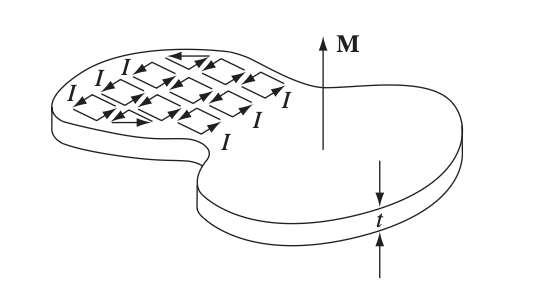
\includegraphics[width=1.0\linewidth]{figure/image55.png}
    \end{subfigure}
    \hfill
    \begin{subfigure}{0.45\textwidth}
        \centering
        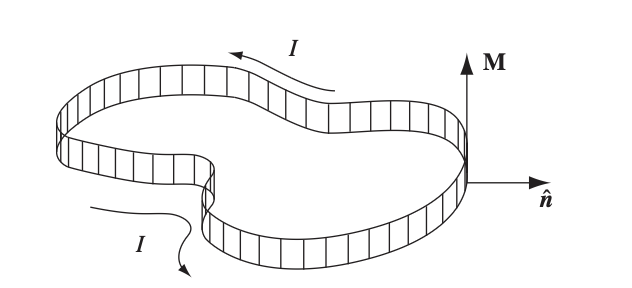
\includegraphics[width=1.0 \linewidth]{figure/image56.png}
    \end{subfigure}
    \caption{}
    \label{Figure:lasta_sottile}
\end{figure}

Se $\mathbf{M}$ è uniforme si nota che tutte le correnti interne si annullano: ogni volta che ce n'è una diretta verso destra, una contigua è diretta verso sinistra. Tuttavia, al bordo non c'è alcuna spira adiacente che possa effettuare la cancellazione. L'intero sistema è quindi equivalente a un unico nastro di corrente $i$ che scorre lungo il contorno.\\

\'E possibile esprimere questa corrente, in termini di $\mathbf{M}$. Supponiamo che ciascuna delle piccole spire abbia area $\Sigma$ e spessore $h$ . In termini della magnetizzazione $M$, il suo momento di dipolo è $m = M \ \Sigma h$. Tuttavia in termine della corrente $i$ vale $m = i \Sigma$. Quindi deve valere $i = Mh$ e quindi si ricava facilmente che 

\begin{equation}
    \mathbf{K}_m = \mathbf{M} \times \mathbf{u}_n
\end{equation}

Che è proprio quello che ci aspettavamo.\\

Quando la magnetizzazione è non uniforme, le correnti interne non si annullano più. 

\begin{figure} [h]
    \centering
    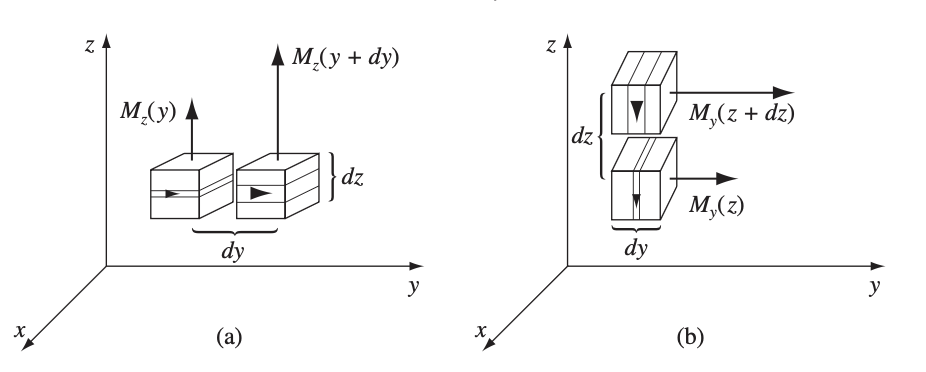
\includegraphics[width=0.75\linewidth]{figure/image58.png}
    \caption{}
    \label{fig:dipolo_non_unif}
\end{figure}

La Figura \ref{fig:dipolo_non_unif} mostra due porzioni adiacenti di materiale magnetizzato, con una freccia più grande su quella a destra che suggerisce una magnetizzazione maggiore in quel punto. Sulla superficie in cui esse si incontrano, c'è una corrente netta nella direzione $x$, data da

\[
i_x = \big[ M_z(y + dy) - M_z(y) \big] \, dz 
= \frac{\partial M_z}{\partial y} \, dy \, dz.
\]

La corrispondente densità di corrente volumica è quindi

\[
(j_m)_x = \frac{\partial M_z}{\partial y}.
\]

Allo stesso modo, una magnetizzazione non uniforme nella direzione $y$ contribuirebbe con un termine $-\partial M_y / \partial z$, per cui

\[
(j_m)_x = \frac{\partial M_z}{\partial y} - \frac{\partial M_y}{\partial z}.
\]

In generale, quindi,

\[
\mathbf{j}_m = \nabla \times \mathbf{M},
\]

in accordo, ancora una volta, con il risultato trovato sopra.

\section{Equazioni della magnetostatica nei mezzi}

Dal momento che il campo magnetico è solinoidale, anche in presenza di mezzi continuano a valere le due condizioni, integrale e locale, date da

\begin{equation*}
    \oint_{\Sigma} \mathbf{B} \cdot \mathbf{u}_n \ d\Sigma = 0 \quad , \quad \nabla \cdot \mathbf{B} = 0 
\end{equation*}

Anche la legge di Ampère rimane valida, \emph{purché si tenga conto delle correnti amperiane oltre che alle correnti di conduzione}:

\begin{tcolorbox}[colback=yellow!10!white, colframe=orange!70!black, boxrule=0.8pt]
\begin{equation}
        \oint \mathbf{B} \cdot d \mathbf{s} = \mu_0 (Ni + i_m)
\end{equation}
\end{tcolorbox}

Deduciamo la forma locale 

\begin{tcolorbox}[colback=yellow!10!white, colframe=orange!70!black, boxrule=0.8pt]
\begin{equation}
        \nabla \times \mathbf{B} = \mu_0 (\mathbf{j} + \mathbf{j}_m)
\end{equation}
\end{tcolorbox}

Allora si nota facilmente che 

\begin{equation}
    \frac{\nabla \times \mathbf{B}}{\mu_0} = \nabla \times \frac{\mathbf{B}}{\mu_0} = \mathbf{j} + \nabla \times \mathbf{M} \implies \nabla \times \left( \frac{\mathbf{B}}{\mu_0} - \mathbf{M} \right) = \mathbf{j}
\end{equation}

A cui corrisponde l'integrale 

\begin{equation}
    \oint \left( \frac{\mathbf{B}}{\mu_0} - \mathbf{M} \right) \cdot d \mathbf{s} = i
\end{equation}

\newpage

Allora possiamo andare a definire una nuova grandezza vettoriale 

\begin{tcolorbox}[colback=yellow!10!white, colframe=orange!70!black, boxrule=0.8pt]
\begin{equation}
        \mathbf{H} = \frac{\mathbf{B}}{\mu_0} - \mathbf{M}
\end{equation}
\end{tcolorbox}

Dove $\mathbf{H}$ prende il nome di \emph{campo magnetizzante}.  \mkeyword{campo magnetizzante}\\

Allora possiamo scrivere:

\begin{tcolorbox}[colback=yellow!10!white, colframe=orange!70!black, boxrule=0.8pt]
\begin{equation}
        \nabla \times \mathbf{H} = \mathbf{j} \quad , \quad \oint \mathbf{H} \cdot d\mathbf{s} = i
\end{equation}
\end{tcolorbox}

La circuitazione del vettore $\mathbf{H}$ lungo una linea chiusa è uguale alla somma delle correnti di conduzione concatenate con la linea; mentre il rotore del vettore $\mathbf{H}$ è uguale alla densità delle correnti di conduzione.\\

La circuitazione del vettore $\mathbf{H}$ non dipende dalla presenza del materiale magnetizzato. \\

\'E possibile trovare una relazione diretta tra $\mathbf{H}$ e $\mathbf{B}$ e tra $\mathbf{H}$ e $\mathbf{M}$. \\
Assumendo come relazione caratteristica 

\begin{tcolorbox}[colback=yellow!10!white, colframe=orange!70!black, boxrule=0.8pt]
\begin{equation}
        \mathbf{M} = \chi_m \mathbf{H} = (\kappa_m - 1) \mathbf{H}
\end{equation}
\end{tcolorbox}

Dove $\kappa_m$ prende il nome di \emph{permeabilità magnetica relativa del mezzo} \mkeyword{permeabilità magnetica relativa del mezzo}, mentre $\chi_m$ prende il nome di \emph{suscettività magnetica}. \mkeyword{suscettività magnetica}\\
Queste due grandezze \emph{dipendono solamente dalla natura del mezzo, indipendentemente dalla geometria e grandezza}. \\

Allora abbiamo come immediata conseguenza

\begin{tcolorbox}[colback=yellow!10!white, colframe=orange!70!black, boxrule=0.8pt]
\begin{equation}
        \mathbf{B} = \mu_0 \kappa_m \ \mathbf{H} = \mu \ \mathbf{H}
\end{equation}
\end{tcolorbox}

Dove $\mu$ è definito come il prodotto tra $\mu_0$ e $\kappa_m$ e prende il nome \emph{permeabilità magnetica assoluta}. \mkeyword{permeabilità magnetica assoluta}\\

\'E possibile trovare una relazione che leghi $\mathbf{M}$ e $\mathbf{B}$

\begin{tcolorbox}[colback=yellow!10!white, colframe=orange!70!black, boxrule=0.8pt]
\begin{equation}
        \mathbf{M} = \frac{\chi_m}{\mu} \ \mathbf{B} = \frac{1}{\mu_0} \frac{\chi_m}{\kappa_m} \mathbf{B} = \frac{1}{\mu_0} \frac{\kappa_m - 1}{\kappa_m} \mathbf{B}
\end{equation}
\end{tcolorbox}

\newpage

\section{Discontinuità dei campi sulla superficie di separazione tra due mezzi magnetizzati}

Prima di andare a vedere come si comporta un campo magnetico quando attraversa una superficie di separazione tra due mezzi con permeabilità magnetica diversa, vediamo come questo si comporta quando nell'attraversamento di una superficie sede di una corrente con densità lineare $\mathbf{K}_s$.  

\begin{figure}[h]
    \centering
    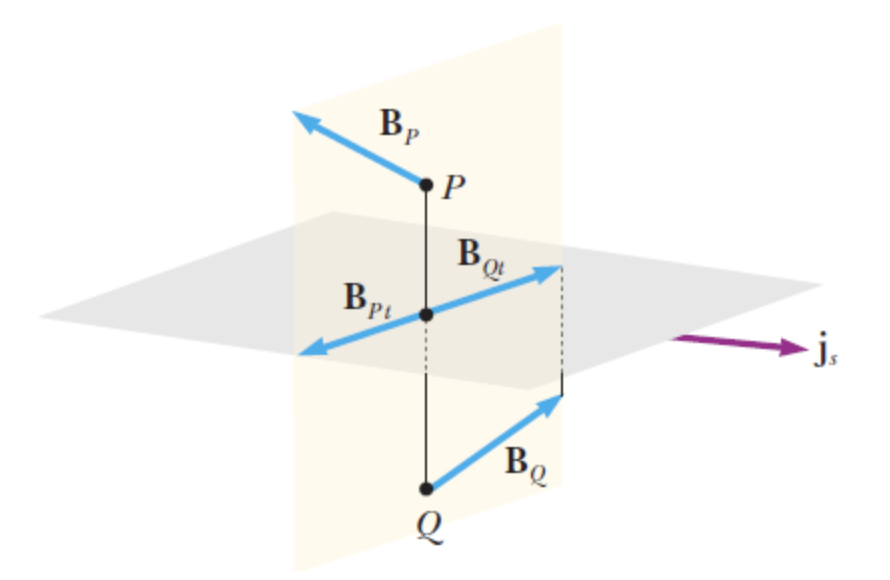
\includegraphics[width=0.7\linewidth]{figure/image59.png}
    \caption{}
    \label{fig:placeholder}
\end{figure}

Presi due punti $P$ e $Q$ molto vicini alla superficie, che quindi localmente appare piana, il campo magnetico dovuto alla corrente superficiale nei punti $P$ e $Q$ è dato dalla relazione 

\begin{equation}
    \mathbf{B} = \frac{\mu_0}{2} \mathbf{K}_s \times \mathbf{u} 
\end{equation}


A questo campo in generale si sovrappone un campo magnetico $\mathbf{B}$ dovuto ad altre sorgenti, che nei punti $P$ e $Q$ molto vicini tra loro ha lo stesso valore. Il campo magnetico totale nei due punti è pertanto diverso:

\begin{equation*}
    \mathbf{B}_P = \mathbf{B} + \frac{\mu_0}{2} \mathbf{K}_s \times \mathbf{u}_n \quad , \quad \mathbf{B}_Q = \mathbf{B} - \frac{\mu_0}{2} \mathbf{K}_s \times \mathbf{u}_n
\end{equation*}

La discontinuità è data da 

\begin{tcolorbox}[colback=yellow!10!white, colframe=orange!70!black, boxrule=0.8pt]
\begin{equation}
        \Delta \mathbf{B} = \mathbf{B}_P - \mathbf{B}_Q = \mu_0 \mathbf{K}_s \times \mathbf{u}_n
\end{equation}
\end{tcolorbox}

Quindi il campo magnetico varia nell'attraversamento di una densità lineare di corrente. \\

\newpage

\subsection{Discontinuità tra mezzi}

Vediamo come questo si comporta quando attraversa una superficie di separazione tra due materiali con permeabilità magnetica diversa.\\

Supponiamo di avere due mezzi con permeabilità magnetica relativa $\kappa_{m1}$ e $\kappa_{m2}$. Indichiamo con $\mathbf{H}_1$, $\mathbf{B}_1 = \mu_1 \mathbf{H}_1$ i campi nel primo mezzo e con $\mathbf{H}_2$, $\mathbf{B}_2 = \mu_2 \mathbf{H}_2$ e sia $\mathbf{u}_n$ la normale alla superficie di separazione nel punto $P$ considerato.\\

\begin{figure} [h]
    \centering
    \begin{subfigure}{0.45\textwidth}
        \centering
        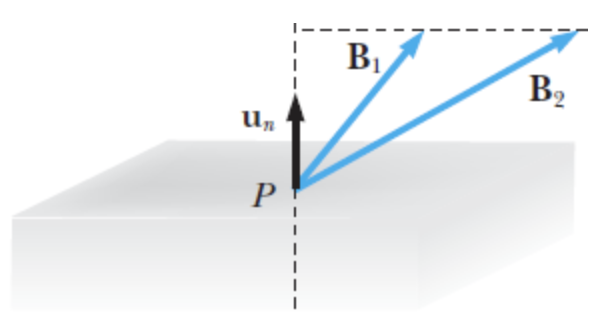
\includegraphics[width=0.80\linewidth]{figure/image60.png}
        \label{fig:placeholder}
    \end{subfigure}
    \hfill
    \begin{subfigure}{0.45\textwidth}
        \centering
        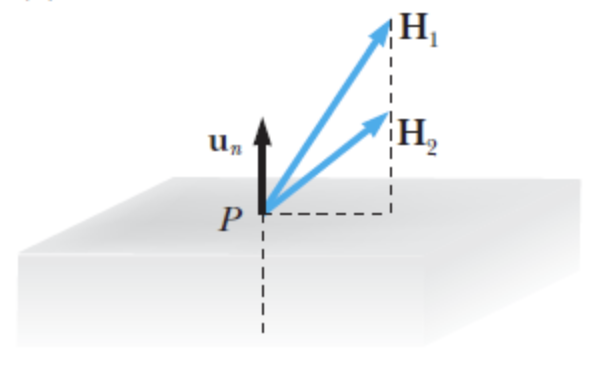
\includegraphics[width=0.80 \linewidth]{figure/image61.png}
    \end{subfigure}
    \caption{}
\end{figure}

Ammettiamo dunque che $\mathbf{H}_1$, $\mathbf{B}_1 = \mu_1 \mathbf{H}_1$, $\mathbf{H}_2$, $\mathbf{B}_2 = \mu_2 \mathbf{H}_2$ siano tutti in uno stesso piano che contiene la normale un alla superficie di separazione nel punto $P$ considerato.\\
L’applicazione della legge di Gauss del campo $\mathbf{B}$ ad una scatola cilindrica di altezza infinitesima, con le basi nei due mezzi e parallele alla superficie, porta alla relazione

\begin{tcolorbox}[colback=yellow!10!white, colframe=orange!70!black, boxrule=0.8pt]
\begin{equation}
        B_{1n} = B_1 \cos \theta_1 = B_2 \cos \theta_2 = B_{2n}
\end{equation}
\end{tcolorbox}

Cioè il campo magnetico $\mathbf{B}$ ha la stessa componente normale dalle due parti della superficie di separazione. \\
Da questa segue 

\begin{tcolorbox}[colback=yellow!10!white, colframe=orange!70!black, boxrule=0.8pt]
\begin{equation}
        \kappa_1 H_1 \cos \theta_1 = \kappa_2 H_2 \cos \theta _2
\end{equation}
\end{tcolorbox}

Applichiamo la legge di Ampère a un rettangolo che sta nel piano individuato dai campi, con due lati paralleli alla superficie di separazione e da parti opposte e gli altri due lati infinitesimi. Si trova

\begin{equation}
    \oint \mathbf{H} \cdot d \mathbf{s}  = H_{1t} h - H_{2t} h = 0
\end{equation}

non essendoci correnti di conduzione concatenate e quindi 

\begin{tcolorbox}[colback=yellow!10!white, colframe=orange!70!black, boxrule=0.8pt]
\begin{equation}
        H_1 \sin \theta_1 =  H_2 \sin \theta _2
\end{equation}
\end{tcolorbox}

Combinando i risultati ottenuti si ottiene

\begin{tcolorbox}[colback=yellow!10!white, colframe=orange!70!black, boxrule=0.8pt]
\begin{equation}
        \frac{\text{tg} \theta_1}{\text{tg}} = \frac{\kappa_{m1}}{\kappa_{m2}}
\end{equation}
\end{tcolorbox}

\section{Confronto tra le leggi dell'elettrostatica e della magnetostatica in mezzi omogenei indefiniti}

Abbiamo già notato varie volte nel corso di questo capitolo analogie con la trattazione delle proprietà dei dielettrici polarizzati. 
La ragione risiede nel fatto che, pur essendo fenomeni fisici diversi, le equazioni che li descrivono hanno la stessa struttura e quindi le soluzioni sono matematicamente eguali, anche se si riferiscono a campi diversi .\\

Per effetture il confronto dove è più appropriato, riscriviamo le equazioni generali dell'elettrostatica e della magnetostatica in mezzi indefiniti e in assenza di cariche elettriche libere ($\rho = 0$) e di correnti di conduzione ($\mathbf{j} = 0$):

\begin{tcolorbox}[colback=yellow!10!white, colframe=orange!70!black, boxrule=0.8pt]
\begin{equation}
\begin{array}{cc}
\nabla \times \mathbf{E} = 0 & \nabla \times \mathbf{H} = 0 \\[1.2em]
\nabla \cdot \mathbf{D} = 0 & \nabla \cdot \mathbf{B} = 0 \\[1.2em]
\dfrac{\mathbf{D}}{\varepsilon_0} = \mathbf{E} + \dfrac{\mathbf{P}}{\varepsilon_0}
&
\dfrac{\mathbf{B}}{\mu_0} = \mathbf{H} + \mathbf{M}
\end{array}
\end{equation}
\end{tcolorbox}

Queste mettono in evidenza le corrispondenze formali

\begin{tcolorbox}[colback=yellow!10!white, colframe=orange!70!black, boxrule=0.8pt]
\begin{equation}
    \mathbf{E} \leftrightarrow \mathbf{H} \quad , \quad \frac{\mathbf{D}}{\varepsilon_0} \leftrightarrow \frac{\mathbf{B}}{\mu_0}  \quad , \quad \frac{\mathbf{P}}{\varepsilon_0} \leftrightarrow \mathbf{M}
\end{equation}
\end{tcolorbox}